\subsection{Calcul de la hauteur d'eau à séparer}
Dans un premier temps, la fonction va calculer la hauteur d'eau présente à la surface de l'unité. Elle se compose de la pluie $P$ (en $m$) ainsi que du débit de ruissellement $Q_{SU}(t-1)$ (en $m\up3/s$) provenant des éventuelles SU situées en amont et calculé au pas de temps précédent.

\begin{equation}
\label{HeightSU}
H = P + \sum_{SU_{up}} \left( \frac{Q_{SU}(t-1) \times \Delta t}{A_{SU}} \right)
\end{equation}


où $H$ est la hauteur d'eau présente à la surface de la SU ($m$), $\Delta t$ est le pas de temps de simulation ($s$), et $A_{SU}$ est la surface de l'unité sur laquelle est effectué le calcul ($m\up2$).


\subsection{Calcul de l'infiltrabilité}
La fonction de production de Morel-Seytoux \cite{MorelS1978} est une adaptation des hypothèses de Green et Ampt \cite{Green1911}. L'hypothèse majeure est la forme rectangulaire du front d'infiltration dans le sol, comme schématisé dans la figure ci-dessous. Le modèle a ensuite été adapté à la structure de MHYDAS par Moussa et al. \cite{Moussa2002}.\\

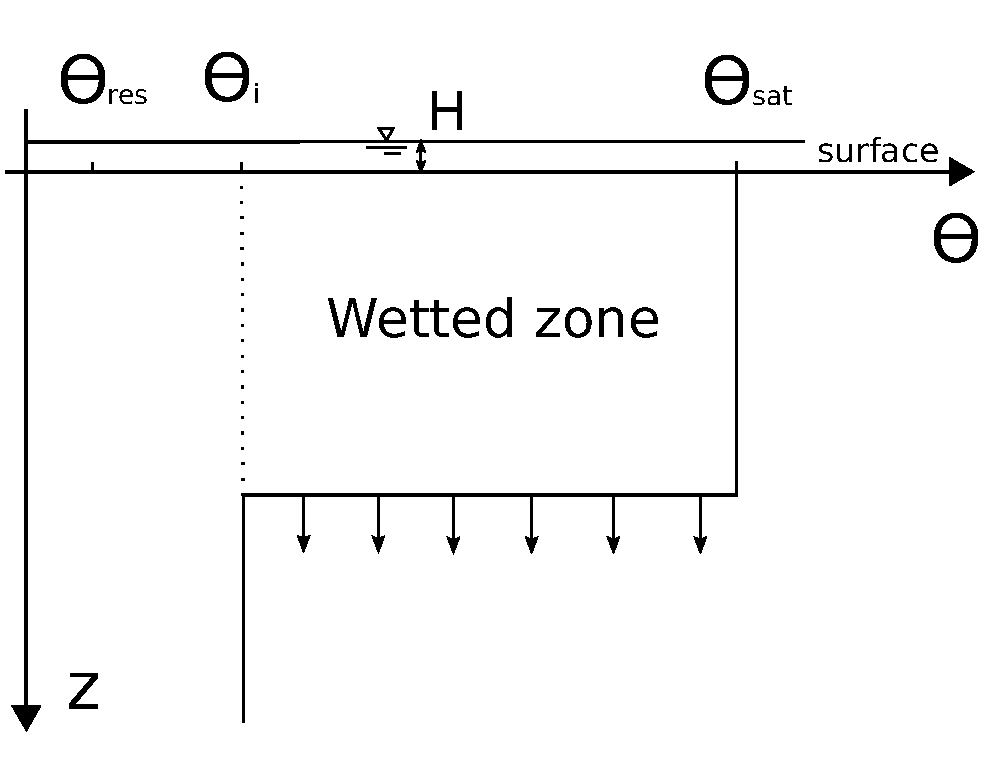
\includegraphics[width=8cm]{common/Green_Ampt_humidity.pdf}\\

Le ruissellement ne peut être observé que si le stock d'eau dans la couche superficielle du sol est à saturation. Ce temps caractéristique est appelé ``temps de flaquage''. Le modèle situe donc le début de l’infiltration maximale en fonction du temps de flaquage $t_p$ : lorsque $t < t_p$ toute la pluie est transformée en infiltration et quand $t > t_p$ il y a production de ruissellement selon l'équation \ref{MSeytoux}. Ce comportement peut être schématisé de la façon suivante avec l'infiltrabilité $f(t)$ ($m/s$) qui diminue au cours du temps à partir de $t_p$ pour tendre vers la conductivité hydraulique à saturation $K_{sat}$.\\

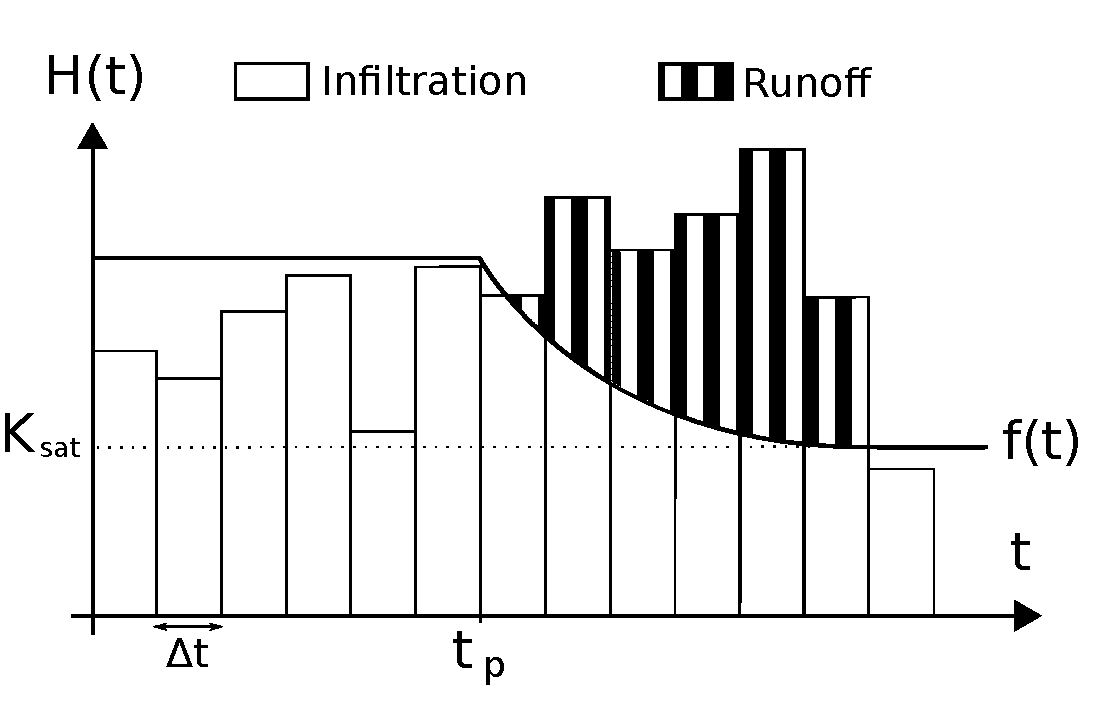
\includegraphics[width=8cm]{common/Separation_infiltration_ruissellement_MSeytoux.pdf}
\begin{equation}
\label{MSeytoux}
\begin{array}{l}
F(t) - F_p - \left(S_f + F_p \times \left(1 - \frac{1}{\beta_{MS}} \right) \right) \times ln \left(\frac{S_f + F(t)}{S_f+F_p} \right)\\
\\
 = \frac{K_s \times (t - t_p)}{\beta_{MS}}
\end{array}
\end{equation}


où $F(t)$ est l'infiltration cumulée au pas de temps $t$ ($m$) et l'intégrale de $f(t)$ représenté sur la figure ci-dessus, $F_p$ est l’infiltration cumulée à $t$ = $t_p$ ($m$), $\beta_{MS}$ est le coefficient de correction visqueuse ($-$) compris entre 1 et 1.7 et généralement pris égal à 1.3 \cite{MorelS1984}, et $K_s$ est la conductivité hydraulique à saturation ($m/s$). $K_s$ est un paramètre distribué sur les unités de surface mais il peut également être variable dans le temps en fonction du travail du sol notamment.\\

Le paramètre $S_f$ ($m$) est un facteur composé de stockage et de succion. L'équation \ref{Sf_equation} qui permet de calculer ce facteur est une approximation de la courbe d'évolution de la hauteur de succion en fonction de la teneur en eau du sol $\phi(\theta)$, ci-après.\\

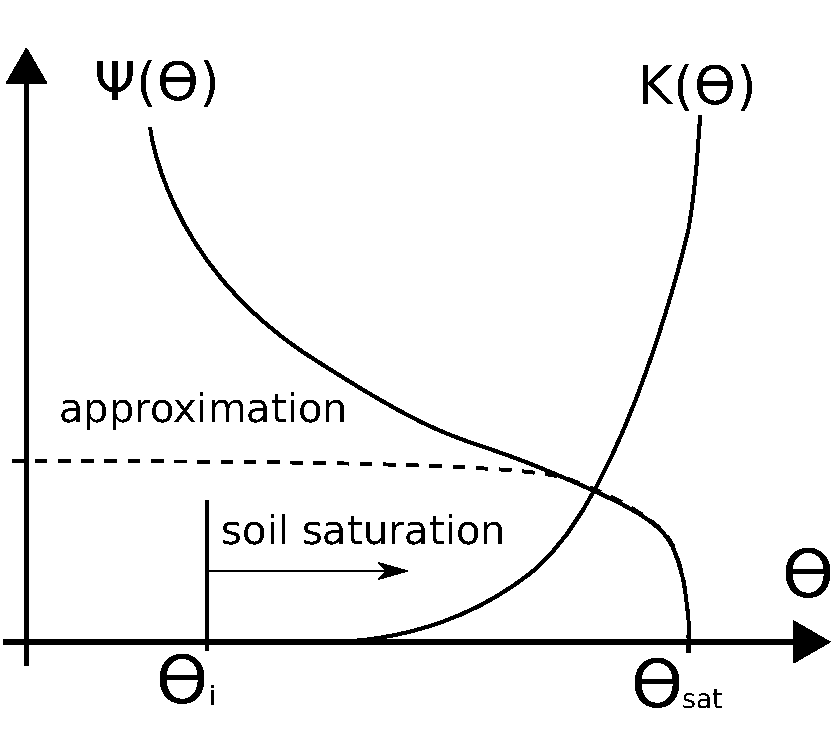
\includegraphics[width=8cm]{common/Sf_approximation.pdf}
\begin{equation}
\label{Sf_equation}
S_f=(\theta_s-\theta_i)\times H_c \times \left(1-\frac{1}{3}\times \left( \frac{\theta_i-\theta_r}{\theta_s-\theta_r} \right) ^6 \right)
\end{equation}


où $Hc$ est la poussée capillaire ($m$), $\theta_s$ est la teneur en eau à saturation ($m\up3 /m\up3$), $\theta_r$ est la teneur en eau résiduelle ($m\up3 /m\up3$) et $\theta_i$ est l’humidité initiale de la couche de surface ($m\up3 /m\up3$). Ce calcul est effectué une seule fois en début de simulation.\\

Pour déterminer l'infiltration cumulée $F(t)$ à chaque pas de temps, la fonction réalise des itérations afin de satisfaire l'équation \ref{MSeytoux}. Le paramètre $ResStep$ (en $m$) traduit la précision de la valeur d'infiltration cumulée calculée. Plus ce paramètre est faible, plus la valeur de $F$ est précise mais plus grand est le nombre d'itérations et donc plus la durée de la simulation sera longue.


\subsection{Calcul de l'infiltration et du ruissellement}
Les variables produites par la fonction sont ensuite calculées de la manière suivante :\\

\hspace{-0.53cm} si $t \le t_p$ : \ \ \ \begin{equation}
\left\{ \begin{array}{l}
   I = H\\
   R = 0
  \end{array}
\right.
\end{equation}\\
\vspace{-0.5mm}
si $t > t_p$ : \ \ \ \begin{equation}
\left\{ \begin{array}{l}
   I = F(t) - F(t-1)\\
   R = H - \left(F(t) - F(t-1) \right)
  \end{array}
\right.
\end{equation}

où $I$ est la hauteur d'eau infiltrée ($m$), $R$ est la hauteur d'eau qui ruisselle à la surface de la SU ($m$), $F$ est l'infiltration cumulée ($m$) au temps $t$, et $H$ est la hauteur d'eau à la surface de la SU ($m$) calculée par l'équation \ref{HeightSU}.\\

La fonction de Morel-Seytoux situant le début du ruissellement à partir du temps de flaquage, une fois que $t_p$ est atteint, le sol ne peut pas être ``désaturé''. C'est pour cette raison que cette fonction ne peut être utilisée qu'à l'échelle événementielle.\\

Des exemples d'utilisation sont disponibles dans la publication de Morel-Seytoux \cite{MorelS1984} et Chahinian \cite{Chahinian2004b} ainsi que dans les thèses de Chahinian \cite{Chahinian2004} et Ghesquière \cite{Ghesquiere2008}.
